
\chapter{Hardware and Software Implementation}\label{sec:methodology}


\section{OSQP}

OSQP (Operator Splitting Quadratic Program) is a \acrshort{qp}-solver developed at the University of Oxford. The main algorithm \cite{osqp}, developed in 2018.

"The algorithm is \acrfull{admm}, using a novel operator splitting technique that
requires the solution of a quasi-definite linear system with the same coefficient matrix
in each iteration." 

Alternating direction method of multipliers solves convex optimization problems using a divide-and-conquer method by breaking the problem up into smaller pieces. It takes the iterative method from the augmented Lagrange method and forces decomposability, giving it a smoother convergence but also a faster runtime.


A shortcoming of this algorithm that is worth mentioning, the convergence time is dependent on the user's choice of step-size parameters. However, the selection of optimal ADMM parameters is still open for discussion\cite{admm_param}. 

Since this algorithm in particular can solve optimization problems to a relative degree of certainty while still using few iterations, therefore being computationally inexpensive, it has been deemed a practical use for embedded processors. 


In addition to the extensive open-source MATLAB interface, it also offers a software package in MATLAB, among others, that can generate C code tailored to a specific quadratic program \cite{osqp-codegen}. This functionality is used in this project to generate C code deigned specifically for the \acrshort{mpc} \acrshort{qp}-problem, and can then be updated at every time step, using the C-interface.

The fact that this solver has both a MATLAB and C code interface, and a code generation software package, made it perfect to use in this project, where both running a simulation in MATLAB, and using  C code in the Simulink model was important. 


\begin{figure}
    \centering
    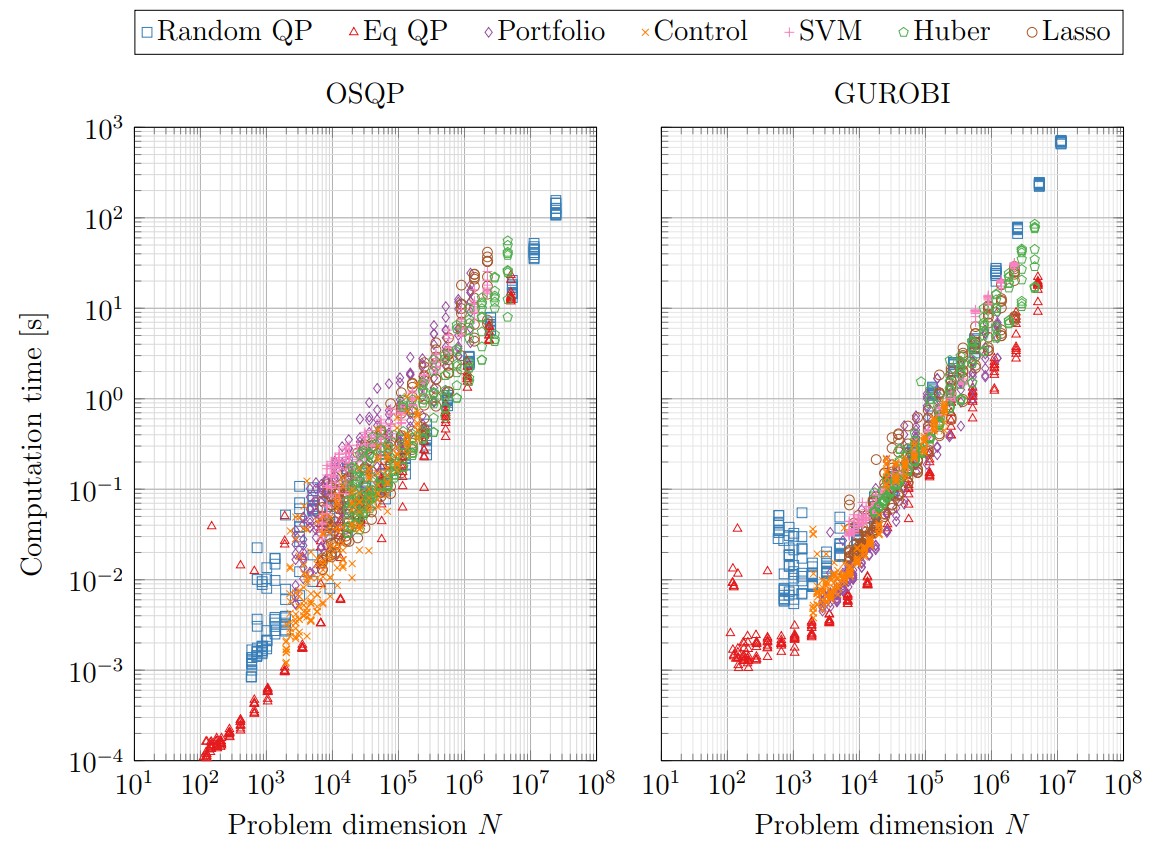
\includegraphics[scale=0.4]{fig/benchmark_osqp.png}
    \caption{Computation time vs problem dimension for OSQP and GUROBI for the 7 benchmark problem classes \cite{osqp}, page 20}
    \label{fig:osqp_benchmark}
\end{figure}

Figure \ref{fig:osqp_benchmark}, taken from \cite{osqp}, demonstrates the computation time of the OSQP-solver and the GUROBI-solver for 7 benchmark problems, and clearly demonstrates OSQP has a clear advantage in most of the problem. Specifically, the optimal control problem which is similar to the online problem for \acrshort{mpc}, performs slightly better with OSQP. 


\section{Simulink Model}

The basis for the Simulink model is the model already written for the helicopter, written by Andreas Flåten for the course TTK4135. 

See appendix \ref{sec:simulink_model_pic} for pictures of the Simulink model.

The helicopter interface \ref{fig:simulink_heli_interface}, pitch and elevation controller \ref{fig:simulink_pitch_contr}, \ref{fig:simulink_elev_contr} and voltage conversion block \ref{fig:simulink_Vd_Vs_block} were taken from the Simulink model used for the Helicopter Lab in TTK4135. 

The additions, are the \acrshort{mpc}-block \ref{fig:MPC} and the estimator \ref{fig:simulink_estimator} which were developed specifically for this project. 

The estimator-block is a Luenberger observer, implemented to estimate the disturbance affecting the system.

was implemented and can be seen here \ref{figure 3}. And the S-Function Builder which contains the \acrshort{mpc} implementation, in C code. 


The S-Function Builder generates the code for the main function of the implementation, and uses the problem description in the file 'workspace.h'. 

It was quickly realized that although the original quadratic program was generated in C code, because of the use of \acrshort{mpc}, this problem changes for every iteration. Both the linear cost $q$ and the upper bound $ub$ depend on the current state of the system $x_0$.

To recalculate the linear cost and the upper bound online, the matrices $bin, cin$ and $f$ had to be defined in C code. Therefore, a simple MATLAB script is used to define the datastructures \verb|c_float bindata[]| as strings in MATLAB and add these to the bottom of the file 'workspace.h', so they can be used by the \acrshort{mpc}-block.

For the version with inequality constraints, $ub$ and $lb$ are the constraints that must be updated. 


\subsection{S-Functions}
MATLAB 2015b is the version of MATLAB used in this project, and the corresponding Simulink version.

S-Functions are one of the functionalities of Simulink that is compatible with QUARC and code generation, so this was used to incorporate OSQP into the Simulink model. 


An S-Function is a Simulink block described in a computer language, in this case,  C. It is documented that S-Functions written in C/C++ are compatible with QUARC, with given known limitations \cite{quarc-s-function}. 

In this project the \textit{S-Function Builder} was used. This Simulink-block automatically generate the C-code necessary for an S-Function, with existing C-code supplied to it. The block generates a wrapper, which is in turn invokes when the model is run. The builder also generates a \verb|.tlc|-file, that describes how to inline the C-code during code generation. 



\section{Hardware In The Loop}

The hardware in the lab is supplied, ready made, by Quanser. 

%https://www.quanser.com/products/3-dof-helicopter/#overview 

The helicopter is a 3 DOF helicopter and is produced and sold by Quanser. along with all the other hardware in the lab. It is a bench top model of a Tandem rotor helicopter %\cite{https://www.quanser.com/products/3-dof-helicopter/#overview}. 
It has two propellers in parallel driven by DC-motors. The helicopter is equipped with three high-resolution encoders to measure the pitch angle between the propellers, the elevation angle, and the travel angle. 

\cite{user_manual_q8_board}
The helicopter is mounted in a slip ring which allows for 360 degree movement in the travel angle.

The hardware controlling the helicopter consists of the Q8-USB 8 Channel USB Data Acquisition Board and the VoltPAQ-X2 2 Channel Linear Voltage Amplifier from Quanser.

The board is an I/O card made for prototyping and Hardware-In-The-Loop development, and receives the signals from the helicopter, which is equipped with sensors. The amplifier receives the system inputs from the written control software supplied by the user and applies voltage to the propellers.


\begin{figure}
    \centering
    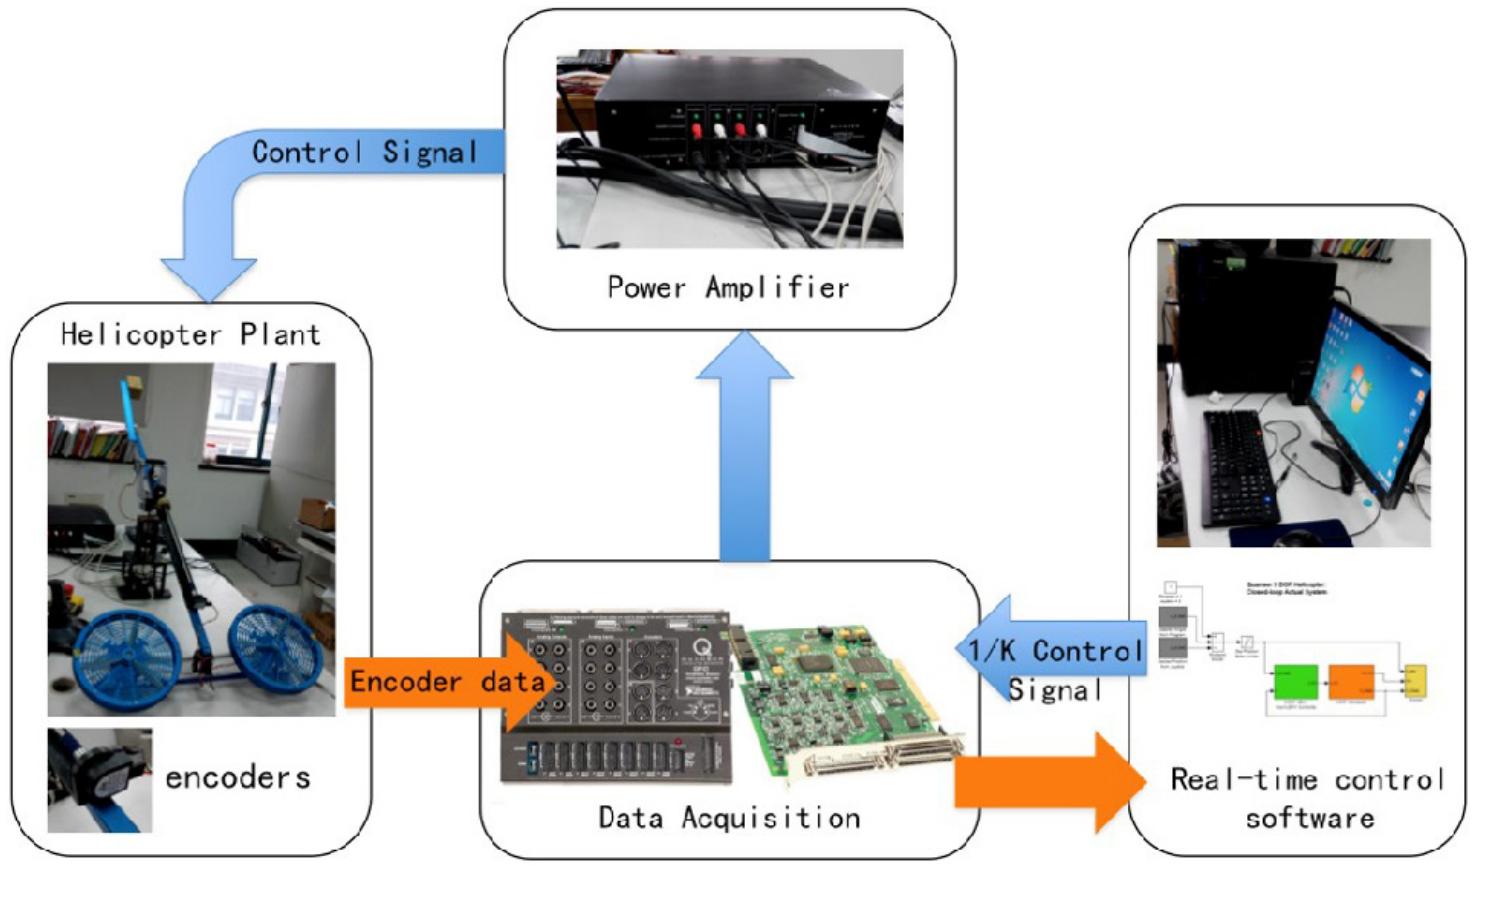
\includegraphics[scale=0.3]{fig/HIL_figure.png}
    \caption{Figure of HIL architecture, stand in}
    \label{fig:hil_architecture}
\end{figure}

Figure \ref{fig:hil_architecture} shows a diagram of the Hardware In The Loop setup. 

\textbf{QUARC}

In addition to the hardware described above, Quanser's 3 DOF helicopter package also comes with QUARC Real-Time Control Software for MATLAB and Simulink. 

"It extends the code generation capabilities of Real-Time Workshop (now called Simulink Coder). It adds a new set of targets the can change the source code generated by Real-Time Workshop to suit the particular platform. QUARC then compiles and links this code with relevant libraries and downloads the code on to the target, which is the Q8 Board. QUARC also has External Mode Communications that allows for connection to the target in Simulink and seeing the signals in real time. 

QUARC has Hardware-In-The-Loop functionality. It has numerous HIL blocks for Simulink, that allows one to use the signals from the board in the Simulink model.

The Simulink blocks written by QUARC that are used in the Simulink model are 
\begin{itemize}
    \item HIL Initialize 
    \item HIL Read Encoder Timebase 
    \item HIL Write Analog
\end{itemize}

There are first for initialization, writing voltage data to the I/O card and reading sensor information from the helicopter so it can be utilized in the Simulink model.

The reading encored block allows for an online visual of all the system signals. Which is why this software is designed for prototyping and testing.


\section{Multi-threading - different sampling times}

\begin{figure}
\centering
\begin{tikzpicture}[every text node part/.style={align=center}]

\draw[black, very thick, ->] (3,1) -- (5,1); %x
\draw[black, very thick, ->] (0,4) -- (0,2); %V_d V_s
\draw[black, very thick, ->] (0,8) -- (0,6); %*u
\draw[black, very thick] (4,1) -- (4,9); %bended arrow 1
\draw[black, very thick, ->] (4,5) -- (3,5); %bended arrow 1
\draw[black, very thick, ->] (4,9) -- (3,9); %bended arrow 2

\draw[black, thick] (-3,0) rectangle (3,2) node[pos=.5] {\Large {Plant (helicopter)}};
\draw[black, thick] (-3,4) rectangle (3,6) node[pos=.5] {\Large{Pitch controller (PD)} \\ \Large{Elevation controller (PID)}};
\draw[black, thick] (-3,8) rectangle (3,10) node[pos=.5] {\Large{MPC}};

\node[anchor=east, text width=4.4] (note1) at (4.8,1.2) {$x$};
\node[anchor=east, text width=4.4] (note2) at (-0.5, 3) {$\m{V_d \\ V_s}$};
\node[anchor=east, text width=4.4] (note2) at (-0.5, 7) {$\m{p_c^* \\ e_c^*}$};
\end{tikzpicture}
\caption{Diagram of system control architecture} \label{fig:system_arch}
\end{figure}

Figure \ref{fig:system_arch} shows a diagram of the system architecture. The highest level of control, the \acrshort{mpc}, should have a lower frequency than the rest of the system, so the lower level controllers have time to reach the given reference value before a new one is calculated.

In a Simulink simulation, a model cannot have modules that are running at different sampling intervals, as Simulink does not support this feature. QUARC, however, does. 

QUARC supports multi-threading, so blocks running on different sampling intervals are simply split into multiple threads, grouped together by sampling rate.  \cite{http://quanser-update.azurewebsites.net/quarc/documentation/quarc_multithreading.html}

When dealing with numerous levels of control, the higher levels of control should run at a lower frequency then the lower levels. 

The \acrshort{mpc} inputs reference values for the lower levels of control, so giving the system a little time to reach the reference before a new one is given, is desirable. 

In this simulation, the lower levels of control have a sampling time of 0.02 seconds, which is 50 Hz. The \acrshort{mpc} is run with 10 Hz, 5 Hz and 2 Hz.

An issue that is encountered when changing the frequency of the \acrshort{mpc} block, is the fact that the model used for the calculation is relatively inaccurate. As mentioned, it is linearized about the equilibrium point, so the inaccuracy increases further away from this point. 

When the frequency of the \acrshort{mpc}-calculations are lower, the system has longer time to develop this inaccuracy before the new state is fed back to the \acrshort{mpc}. This causes an oscillation in both the system and the optimal first state at each timestep. A suggested solution to this problem is using nonlinear model predictive control. This would lead to more accurate control without needing to run the higher level of control at such a high frequency. This is discussed further in chapter \ref{ch:discussion}, after the results from this phenomenon are presented.  



\section{Generating the \acrshort{mpc} problem}

The constraints for $x \in \mathbb{R}^n$ and $u \in \mathbb{R}^m$ are implemented as 
\begin{equation}
    \begin{split}
        Cx + Du \leq e \: \: , \\
        G x_n \leq h \: \: , \\
        C, G \in \mathbb{R}^{a\times n}, \: \: D \in \mathbb{R}^{a \times m} \: \: ,
    \end{split}
\end{equation}
with $a$ being the number of constraints.

With the constraint of the form $\bar C \bm x + \bar D \bm \leq \bar e$, this becomes
\begin{equation}
    \begin{split}
        &\m{C & & & \\
            & C & &   \\
             & & \ddots  & \\
             &  & & C \\
             & & & G} \bm x + \m{D & & & \\
            & D & &  \\
             & & \ddots &  \\
             &  & & D \\
             0 & 0 & \hdots & 0} \bm u \leq \m{e \\ e \\ \vdots\\ e \\ h}\: \: .
    \end{split}
\end{equation}

Inserting $x = S_u u + S_x x_0$, results in 
\begin{equation}
    \begin{split}
        &\bar C(S_u u + S_x x_0) + \bar D u \leq e \: \: , \\
        &\bar C S_u u + \bar C S_x x_0 + \bar D u \leq e \: \: , \\
        &(\bar C S_u + \bar D) u \leq \bar e - \bar C S_x x_0 \: \: .
    \end{split}
\end{equation}

Since $x_0$ is a variable, in the sense that it changes for every timestep, therefore for every call of the online calculations, the constraints are split up as follows,

\begin{equation}
    A_{in} x \leq b_{in} + c_{in} \cdot x_0 \: \: ,
\end{equation}
where
\begin{equation}
    A_{in} = \bar C S_u + \bar D\: \: , b_{in} = \bar e \: \: , c_{in} = -\bar C S_x \: \: .
\end{equation}



The MATLAB implementation of this can be found in listing \ref{lst:gen_mpc}. 


\subection{Calculating the terminal constraint}

The theory for terminal constraints was presented in \ref{sec:terminal_constraint}. There are many ways of approximating this, depending on the complexity of the system. In this implementation, the maximal control invariant set was used for the terminal constraint. 


\begin{equation}
    \m{1 & 0 & 0 & 0 & 0 & 0 & 0 & 0 \\
       -1 & 0 & 0 & 0 & 0 & 0 & 0 & 0 \\
       0 & 0 & 1 & 0 & 0 & 0 & 0 & -1 \\
       0 & 0 & -1 & 0 & 0 & 0 & 0 & -1 \\
       0 & 0 & 0 & 0 & 0 & 1 & 0 & 0\\
       0 & 0 & 0 & 0 & 0 & -1 & 0 & 0 \\
       0 & 0 & 0 & 0 & 0 & 0 & 0 & 1 \\
       1.3 & 3.9 & -2 & -0.6 & 0 & 0 & 0 & 0 \\
       -1.3 & -3.9 & 2 & 0.6 & 0 & 0 & 0 & 0 \\
       1 & 0.08 & 0 & 0 & 0 & 0 & 1 & 0 \\
       -1 & -0.08 & 0 & 0 & 0 & 0 & -1 & 0 \\
       0 & 0 & 1 & 0.08 & 0 & 0 & 0 & 0 \\
       0 & 0 & -1 & -0.08 & 0 & 0 & 0 & 0 \\
       0 & 0 & 0 & 0 & -0.03 & 0.9 & 0 & 0 \\
       0 & 0 & 0 & 0 & 0.03 & -0.9 & 0 & 0 \\
       1.1 & 3.3 & -1.6 & -0.5 & 0 & 0 & 1.3 & 0 \\
       -1.1 & -3.3 & 1.6 & 0.5 & 0 & 0 & -1.3 & 0} \m{\lambda \\ \dot \lambda \\ p \\ \dot p \\ e \\ \dot e \\ d \\ \epsilon_p} \leq \m{3.7 \\ 3.7 \\ 0.5 \\ 0.5 \\ 10000 \\ 10000 \\ 0 \\ 0.4 \\ 0.4 \\ 3.7 \\ 3.7 \\ 0.5 \\ 0.5 \\ 1000 \\ 1000 \\ 0.4 \\ 0.4}
\end{equation}

\section{MATLAB Simulation}